%%==================================================
%% chapter03.tex for TJU Master Thesis
%% Encoding: UTF-8
%%==================================================

\chapter{软管拉伸实验}
\section{引~言}
对软管组件进行拉伸实验,而不是进行内压实验,这是一个综合考虑各方面因素的结果。
首先,进行实验的目的是为了得到准确可靠的数据,以支撑理论模型,这就要求实验环境安全、可控,干扰的变量较少,所需数据如编织角、伸长量可以直接测量。
进行拉伸实验所需要的设备仅为力学万能试验机,安全可控,容易操作。
如果进行内压实验,实验的操作就必须在液压实验台上进行。根据试件的性能,内压荷载需要达到几十兆帕才能发生明显可测的变形。
%学者实验 研究
整个过程风险较大,液压试验台必须加盖隔离保护操作人员,因而液压实验中不能直接接触试件,需要通过额外的设备进行观测。

本文进行了多次拉伸实验,一方面是为了消除实验的系统误差,提高数据的可信度;另一方面,也是由于在理论研究过程中,发现了额外需要关注的部分、对象,也是一个循序渐进的探索过程。本章将着重介绍实验的结果以及对其结果的分析。
\section{观测数据及方法}


\subsection{编织角}
在实验过程中记录编织角并不简单,例如 ,本研究原计划采用摄像法记录软管组件编织角的变化,但由于软管编织层为为曲面,用平面的照片来进行编织角的采样,效果并不理想。测量的结果误差一般在$ \pm $2\textdegree 左右;整个拉伸实验过程中编织角的变化约为20\textdegree 。因此简单的摄像测量法相对误差保守估计在10\%左右。而且,产生误差的因素也很多,包括摄像设备与试件的相对位置,照片成像的质量,测量采样的位置等。因此国外有研究专门开发了记录编织角变化的试验台设备, \citeauthor{Leung2013}\cite{Leung2013}开发了双显微镜头的光学记录设备,
如\ref{fig:dic}图所示,配有伺服驱动装置,可以随着拉伸的过程同步移动,观测某一定点的编织角变化;并采用了数字图像处理技术(digital image corelation, DIC)对观测的结果进行处理,消除了曲面以及摄像角度的影响。

\begin{figure}[!htbp]
	\centering
	\subfigure[]{
		\includegraphics[width=0.4\linewidth]{figure/experiment/dic-1}}		
	\hspace{1cm}
	\subfigure[]{
		\includegraphics[width=0.4\linewidth]{figure/experiment/dic-2}}
	\fcaption{数字化编织角观测设备}{DIC system of braid angle}
	\label{fig:dic}
\end{figure}

本研究由于设备有限,因而采用了另外一种处理方案来解决以上的问题。通过对目标区域进行染色处理,如图 所示,利用编织层表面凹凸不平的特性,趁染色涂料未干之际将编织角拓印在纸张上。

文献未见有类似的方法。从结果上来看,拓印法取得的编织角效果令人满意。拓印的编织纹路如图 所示,可以手工处理,也可通过电脑扫描后利用DIC软件处理,相比复杂的三位结构和空间几何透视关系,这种平面的纹路显然要更加容易处理。

\begin{figure}[!htbp]
	\centering
	\subfigure[]{
		\includegraphics[width=0.2\linewidth]{"figure/experiment/hose-angle-testing"}}		
	\hspace{1cm}
	\subfigure[]{
		\includegraphics[width=0.4\linewidth]{"figure/experiment/hose-angle-testing-2"}}
	\fcaption{占位图}{place holder}
%	\label{fig:placeholder}
\end{figure}

根据实验的经验,拓印记录编织角的纹路后,手工处理数据需要以下几步操作:
\begin{compactenum}
\item 观察两组不同方向的纹路,绘制两条参考线,保证分别与两个方向的纹路保持平行;
\item 测量不同数据点同荷载状态下,拓印纹路的参考线的夹角,计算平均值;
\item 若某组参考线的夹角明显不同于其余数据点,观察参考线绘制是否有误。
\end{compactenum}





\subsection{管径}
拉伸试验中,软管组件的管径会变小,是一个变化较明显的参数。管径测量较为简便,实验中采用游标卡尺即可测量。同样需要在测量编织角的数据点多次测量,过程中也要进行测量。
管径的作用主要是用以衡量标定有限元模型。
\subsection{支座反力与伸长量}
支座反力由试验机测得,一般不需要人为干预,软硬件都相对成熟。需要注意的时一般万能试验机可以记录的数据种类非常丰富,本实验中仅需记录支座反力与支座位移的关系曲线。
一般最大荷载较小的万能试验机测量精度较高,合理地选择试验机,将能得到更为准确的数据。







\section{实验设备}

力学万能试验机


\begin{figure}[!htbp]
	\centering
	\subfigure[]{
		\includegraphics[width=0.4\linewidth]{figure/experiment/tensile-machine}}		
	\hspace{1cm}
	\subfigure[]{
		\includegraphics[width=0.25\linewidth]{figure/experiment/tensile-machine-2}}
	\fcaption{占位图}{place holder}
%	\label{fig:placeholder}
\end{figure}


\section{实验步骤}

\begin{compactenum}
	\item 将软管安装至万能试验机,一般软管组件的的接头较为粗大,需要通过公装连接试验机夹具;
	\item 开始拉伸实验,加载速度不能超过10mm/min;
	\item 工程应变每增加0.05,至少记录一组数据,
	\begin{compactitem}
		\item 支座反力和软骨啊伸长量有试验机系统记录;
		\item 用拓印法记录编织角,至少3个染色区域,分别拓印记录;
		\item 记录染色区域的管径变化;
		\item 记录数据时拉伸的过程不会停止,必须短时间内测量记录各组数据,保证数据具有可比性。
	\end{compactitem}
	\item 试件破坏,实验结束。
\end{compactenum}





\section{第一次拉伸实验}
\subsection{试件参数}
第一次拉伸实验共进行了三组,分别为图\ref{fig:experiment-1-specimen}中芯棒1、芯棒2、芯棒3,“芯棒”代表试件事先编织于芯棒之上,然后抽出芯棒制制成仅有编织层的软管。其编织角由于抽拔芯棒的过程,导致编织角大幅小于平衡角。



\begin{figure}[!htbp]
	\centering
	\subfigure[]{
		\includegraphics[width=0.35\textwidth]{figure/experiment/E1/specimen/E1-1}}
	\hspace{1cm}
	\subfigure[]{
		\includegraphics[width=0.35\textwidth]{figure/experiment/E1/specimen/E1-2}}
	
	\subfigure[]{
		\includegraphics[width=0.35\textwidth]{figure/experiment/E1/specimen/E1-3}}
	\hspace{1cm}
	\subfigure[]{
		\includegraphics[width=0.35\textwidth]{figure/experiment/E1/specimen/E1-4}}
	\fcaption{第一次拉伸实验}{experiment-1}  
	\label{fig:experiment-1-specimen}
\end{figure}

\begin{table}[!htbp]
	\centering
	\fcaption[tab:hosepressurelevle]{实验试件}{实验试件}{Table}{Hose Specimen of the traction experiment}
	\label{tab:hose-specimen}
	\begin{tabular*}{0.8\textwidth}{@{\extracolsep{\fill}}>{\hspace{0.5cm}}cccc}
		\toprule
		                  &     编织层-1     &     编织层-2     &     编织层-3     \\ \midrule
		外径(mm)            &     7.60      &     7.59      &     7.60      \\
		内径 (mm)           &     6.80      &     6.77      &     6.81      \\
		长度 (mm)           &     320.0     &     321.0     &     320.5     \\
		编织角 (\textdegree) &     42.1      &     41.9      &      43       \\
		股数$ \times $根数    & 24$ \times $6 & 24$ \times $6 & 24$ \times $6 \\
		钢丝直径(mm)          &      0.2      &      0.2      &      0.2      \\ \bottomrule
	\end{tabular*} 
\end{table}







\begin{figure}[!htbp]
\centering
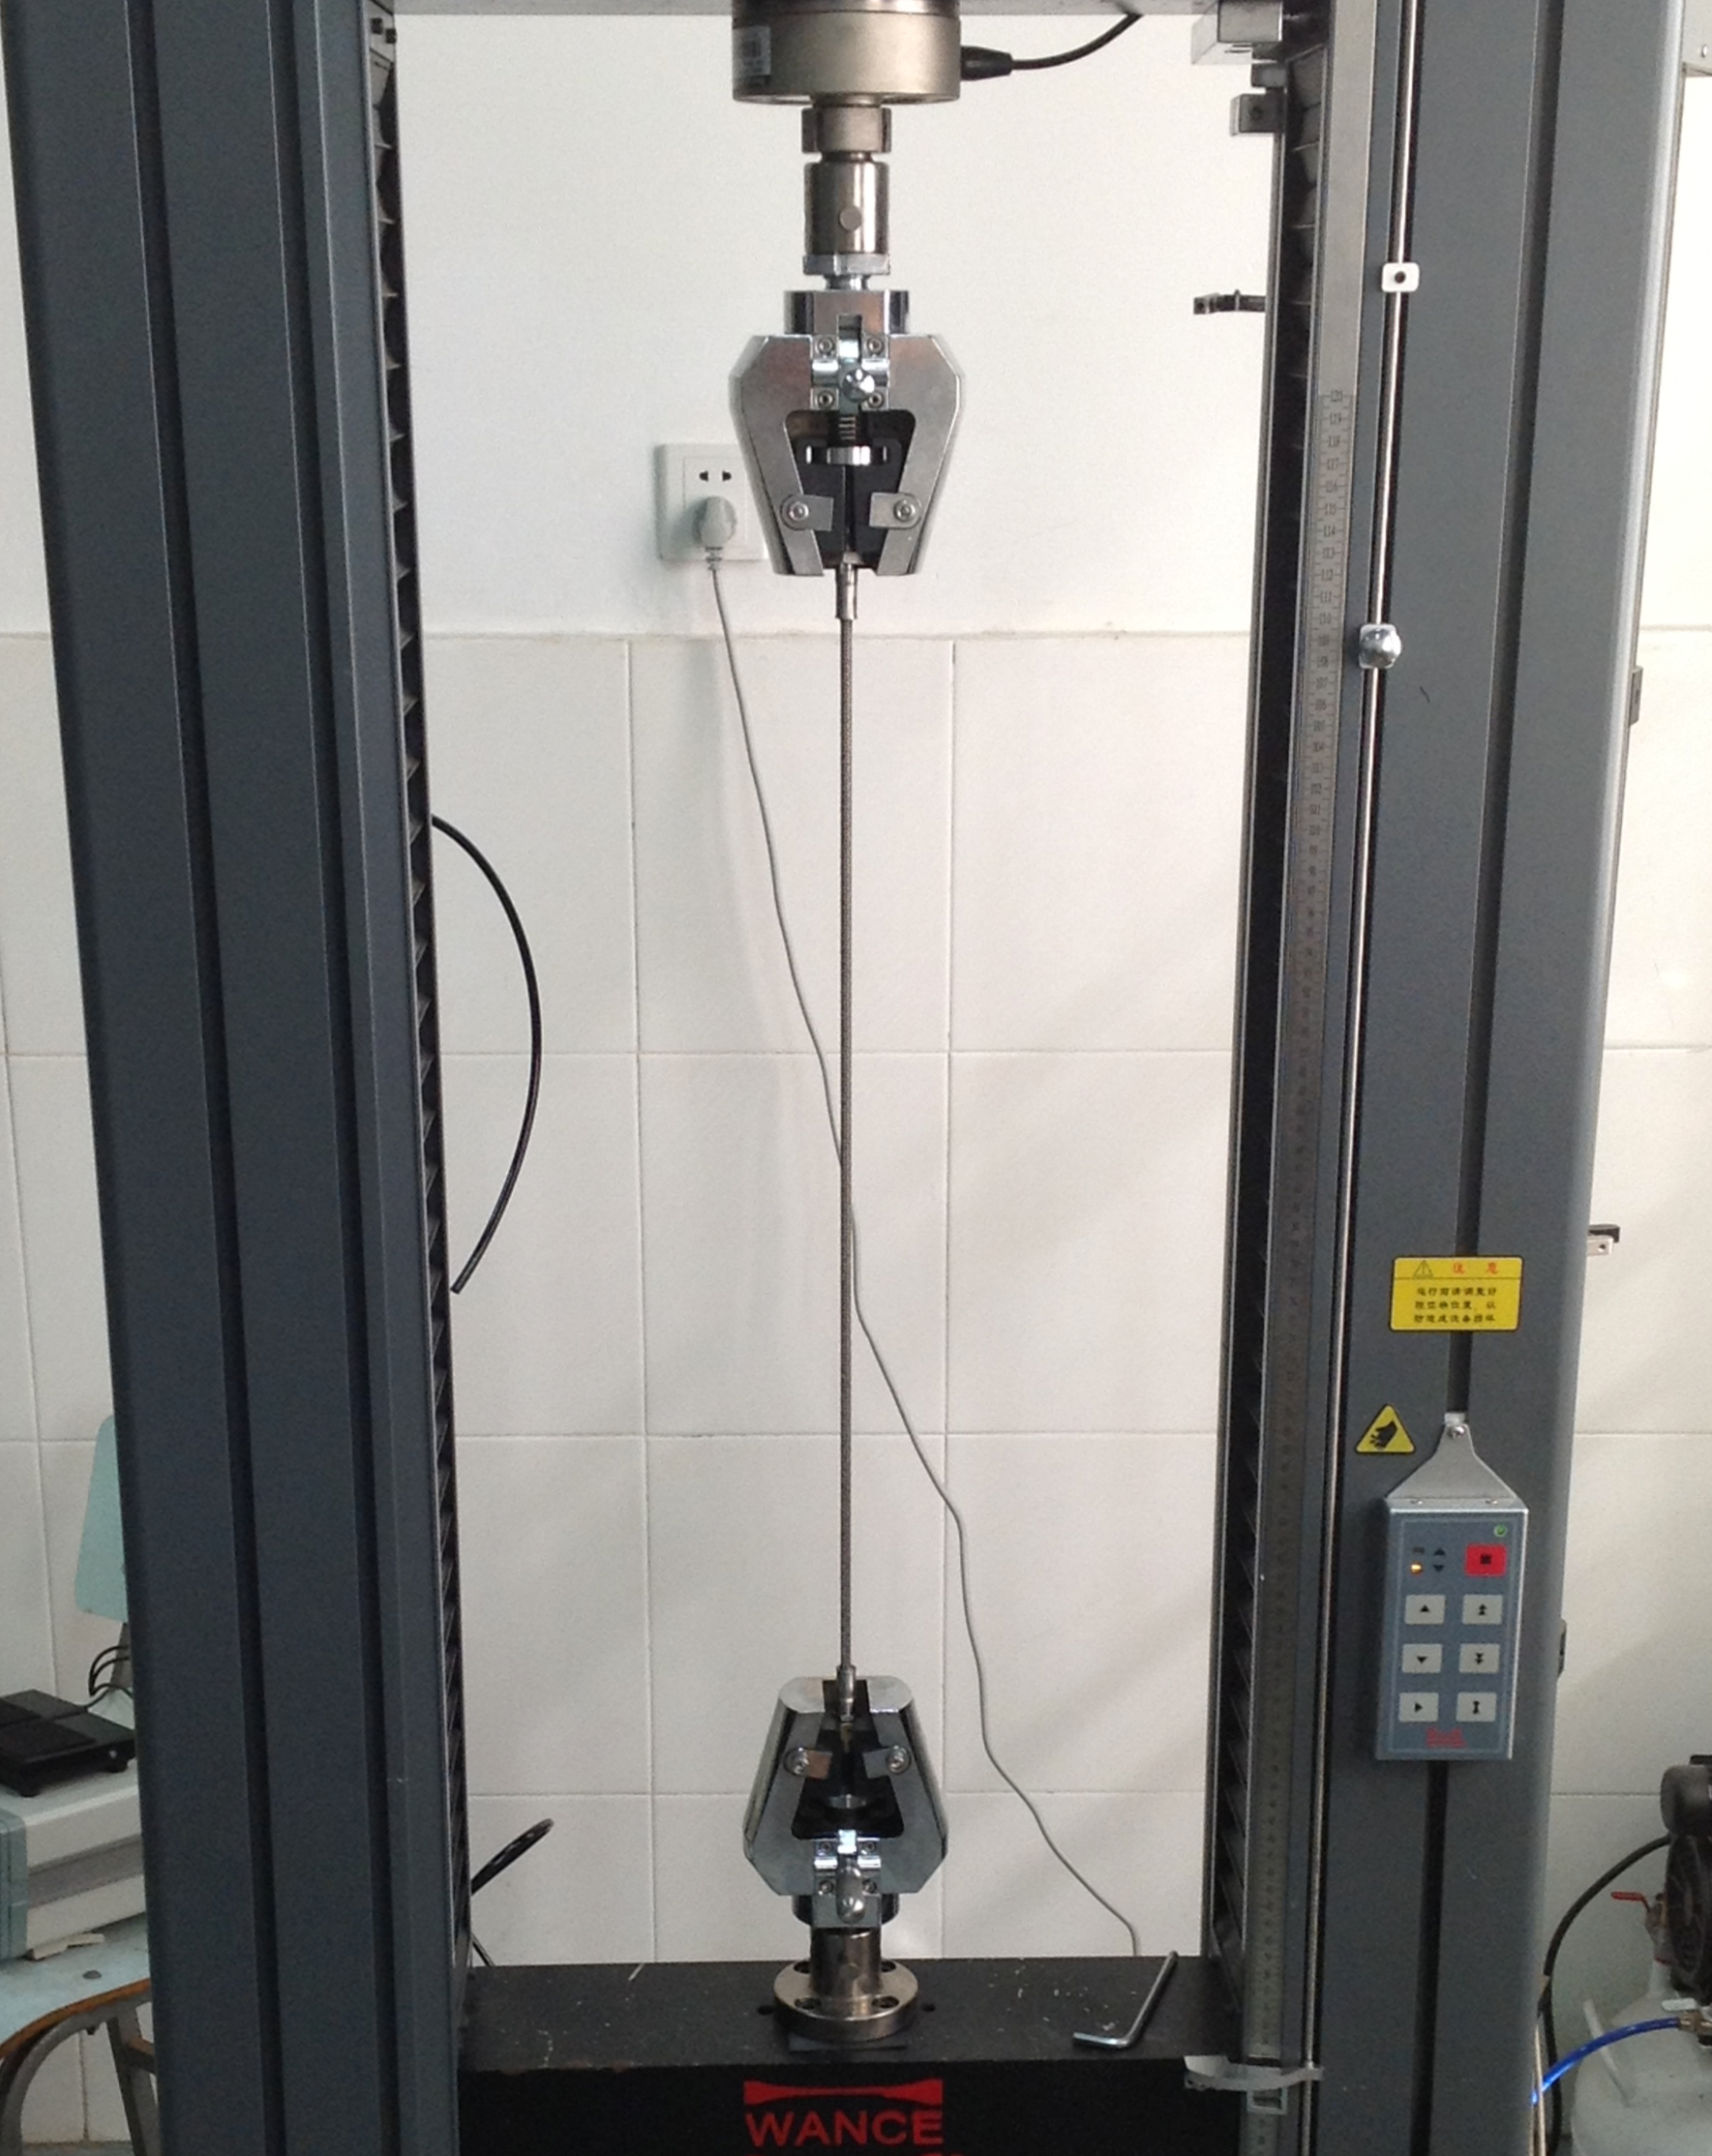
\includegraphics[width=0.4\linewidth]{figure/experiment/tensile}
	\fcaption{第一次拉伸实验}{experiment-1}  
	\label{fig:experiment-1}
\end{figure}






\subsubsection{力位移曲线}
\begin{figure}[!htbp]
	\centering
	\includegraphics[width=0.6\textwidth]{figure/experiment/E1/Graph01}
	
	\subfigure[]{
		\includegraphics[width=0.3\linewidth]{figure/experiment/E1/Graph03}}
	\subfigure[]{
		\includegraphics[width=0.3\linewidth]{figure/experiment/E1/Graph04}}
	\subfigure[]{
		\includegraphics[width=0.3\linewidth]{figure/experiment/E1/Graph05}}
	
	\fcaption{第一次拉伸实验}{experiment-1}  
%	\label{fig:experiment-1}
\end{figure}



\subsubsection{破坏形式}


\begin{figure}[!htbp]
	\centering
	\subfigure{
		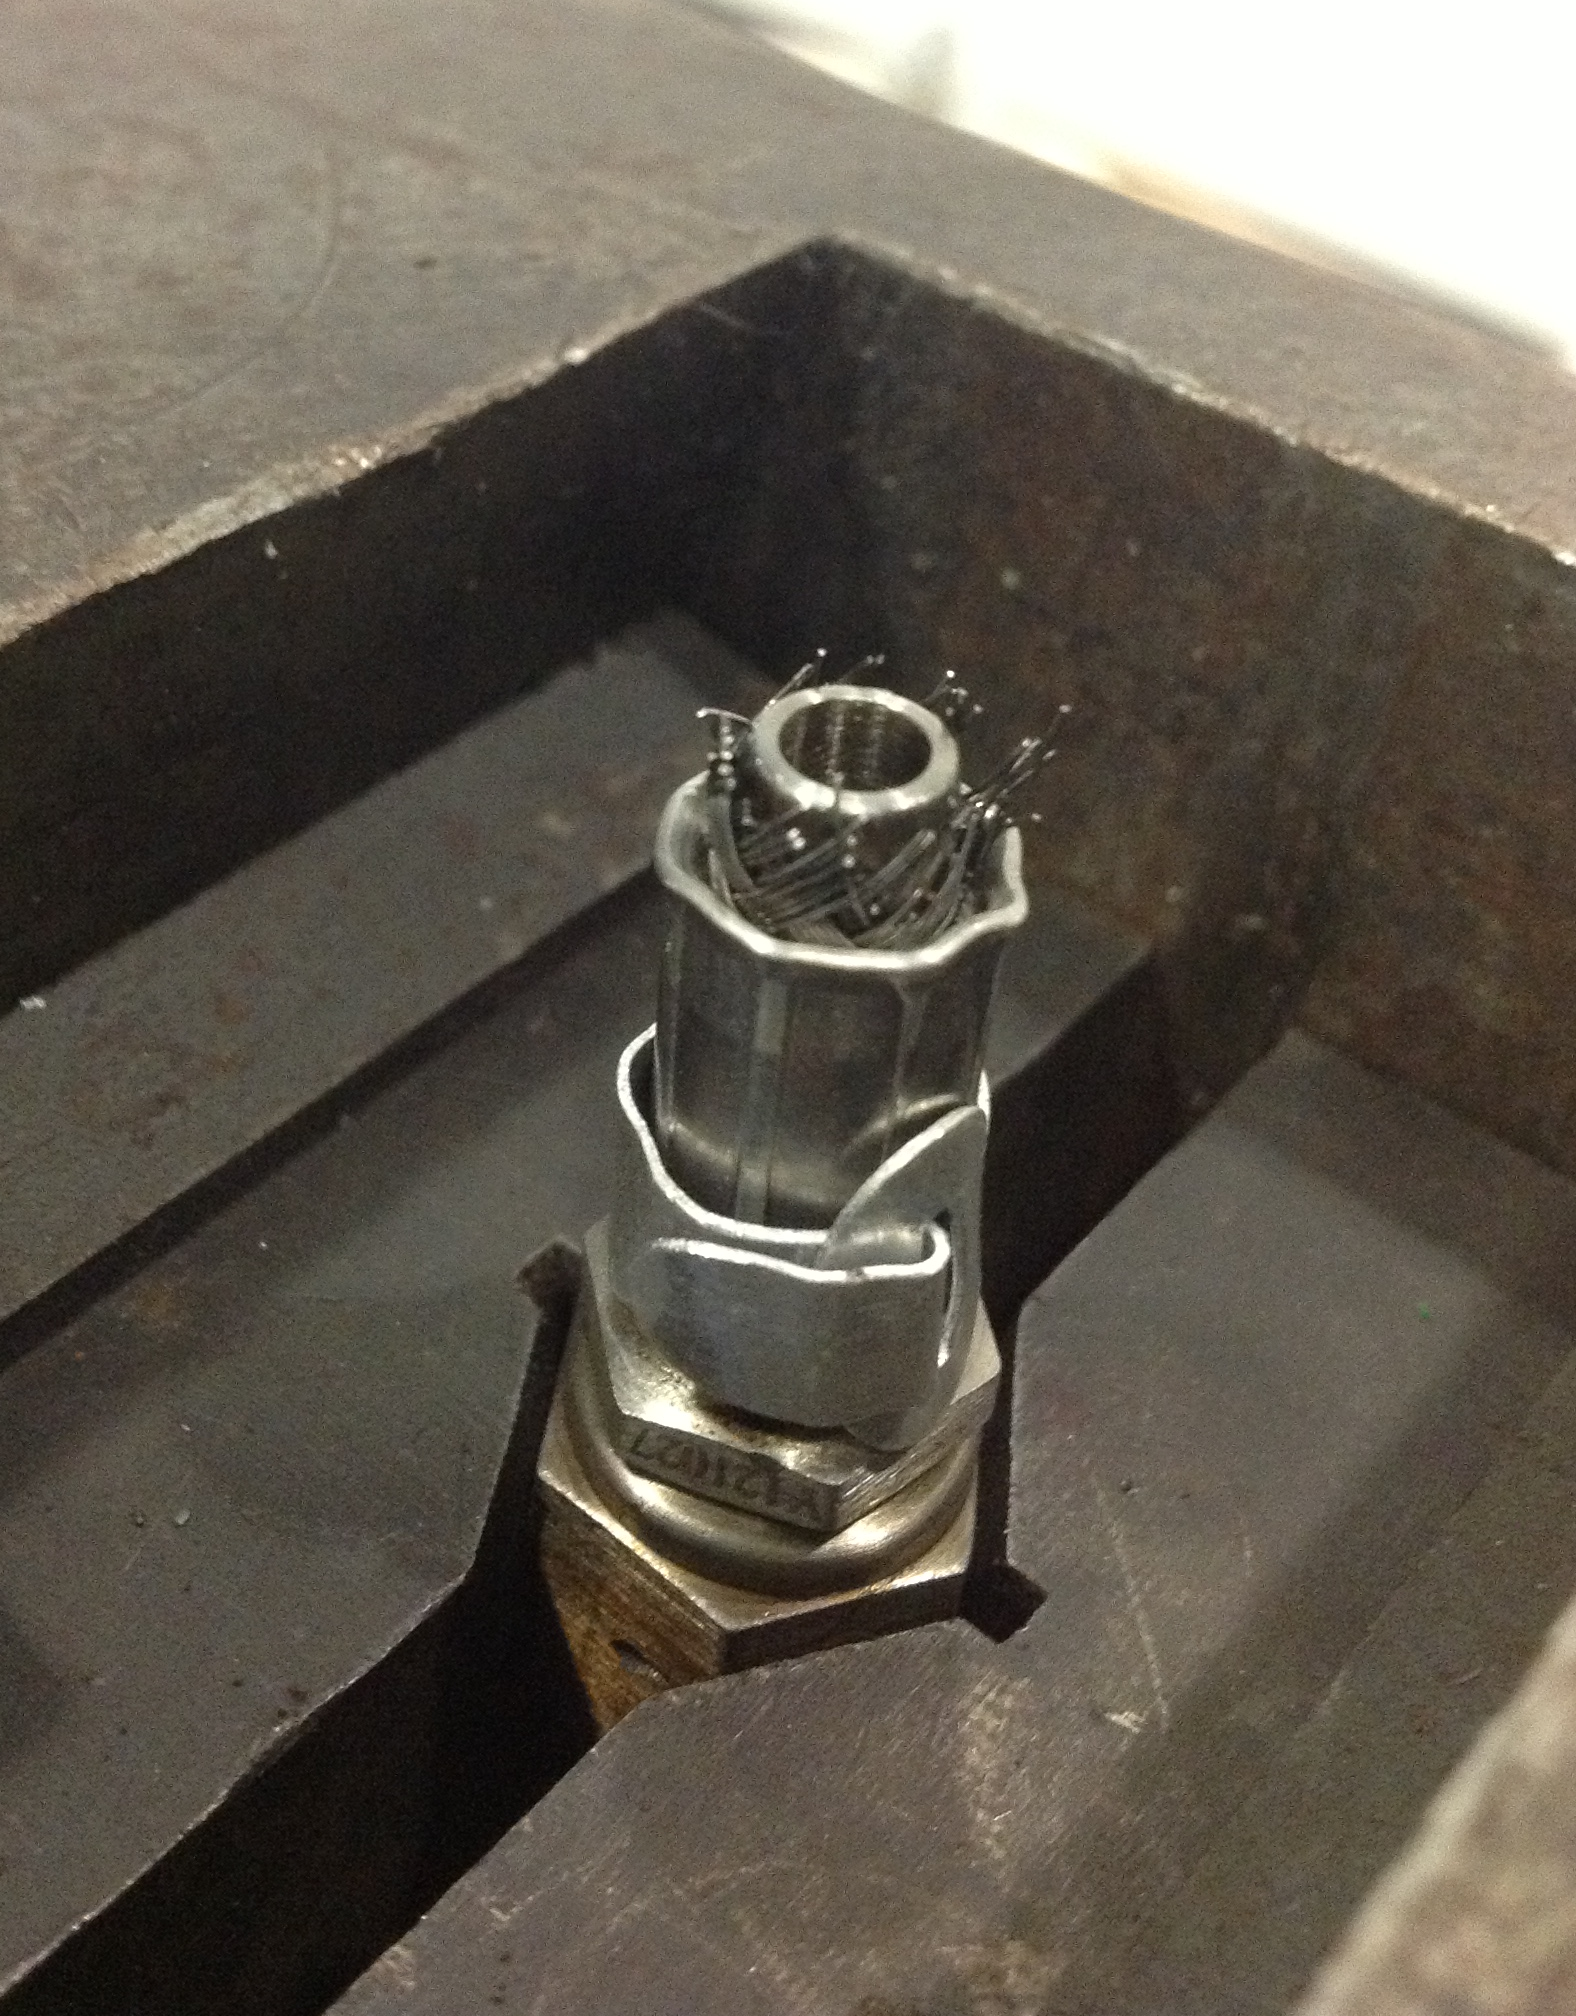
\includegraphics[width=0.35\textwidth]{figure/experiment/E1/failure-1}}
	\hspace{1cm}
	\subfigure{
		\includegraphics[width=0.4\textwidth]{figure/experiment/E1/failure-2}}
	\fcaption{破坏形式}{experiment-1:}
%	\label{fig:experiment-1}
\end{figure}









\subsection{第二次拉伸实验}


\begin{figure}[!htbp]
	\centering
	\includegraphics[width=0.6\textwidth]{figure/experiment/E2/Graph02}
	\fcaption{第二次拉伸实验}{experiment-2}  
	\label{fig:experiment-2}
\end{figure}





\newpage
\subsection{第三次拉伸实验}

\paragraph{第一组试件}

第一组试件

\begin{figure}[!htbp]
	\centering
	
	\subfigure{
		\includegraphics[width=0.5\textwidth]{figure/experiment/E3-G1/Graph01}}
	\subfigure{
		\includegraphics[width=0.6\textwidth]{figure/experiment/E3-G1/Graph02}}
	
	\fcaption{软管组件}{Hose Assembly}  
	\label{fig:hose}
\end{figure}

\paragraph{第二组试件}

第二组试件
\begin{figure}[!htbp]
	\centering
	
	\subfigure{
		\includegraphics[width=0.4\textwidth]{figure/experiment/E3-G2/Graph01}}
	\subfigure{
		\includegraphics[width=0.6\textwidth]{figure/experiment/E3-G2/Graph02}}
	
	\fcaption{软管组件}{Hose Assembly}  
%	\label{fig:hose}
\end{figure}




\paragraph{第三组试件}

第三组试件
\begin{figure}[!htbp]
	\centering
	
	\subfigure{
		\includegraphics[width=0.4\textwidth]{figure/experiment/E3-G3/Graph01}}
	\subfigure{
		\includegraphics[width=0.6\textwidth]{figure/experiment/E3-G3/Graph02}}
	
	\fcaption{软管组件}{Hose Assembly}  
%	\label{fig:hose}
\end{figure}
\paragraph{第四组试件}

第四组试件
\begin{figure}[!htbp]
	\centering
	
	\subfigure{
		\includegraphics[width=0.4\textwidth]{figure/experiment/E3-G4/Graph01}}
	\subfigure{
		\includegraphics[width=0.6\textwidth]{figure/experiment/E3-G4/Graph02}}
	
	\fcaption{软管组件}{Hose Assembly}  
%	\label{fig:hose}
\end{figure}
